% !TeX spellcheck = en_GB
% !TeX encoding = UTF-8
% !TeX root = ../thesis.tex
\chapter{N-gram Bug Detection in \scratch{}}\label{chap:methods}

\begin{figure}[hbtp]
\centering
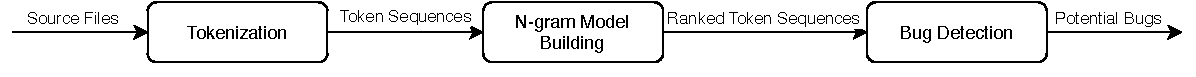
\includegraphics[scale=0.75]{images/Overview.pdf}
\caption{Overview of the n-gram model building process.}
\label{fig:overview}
\end{figure}

Figure \ref{fig:overview} visualises the \ngram{} building process which is explained in this chapter in more detail. In Section~\ref{sec:tokenization} the tokenization process is described with the way the \scratch{} project is parsed and converted into tokens. The next step is to use the created tokens to build the \ngram{} like it is shown in Section~\ref{sec:model}. Finally, bugs can be detected with the help of the calculated model according to Section~\ref{sec:detection}.

\section{Tokenization of \scratch{} Code}\label{sec:tokenization}

\begin{definition}[Token]\label{def:token}
    %
    ``A token is a single fragment of \scratch{} code that is used to partition code into smaller pieces in order to obtain information about its syntax on a specific granularity level.''
    %
\end{definition}

\begin{figure}[hbtp]
\centering
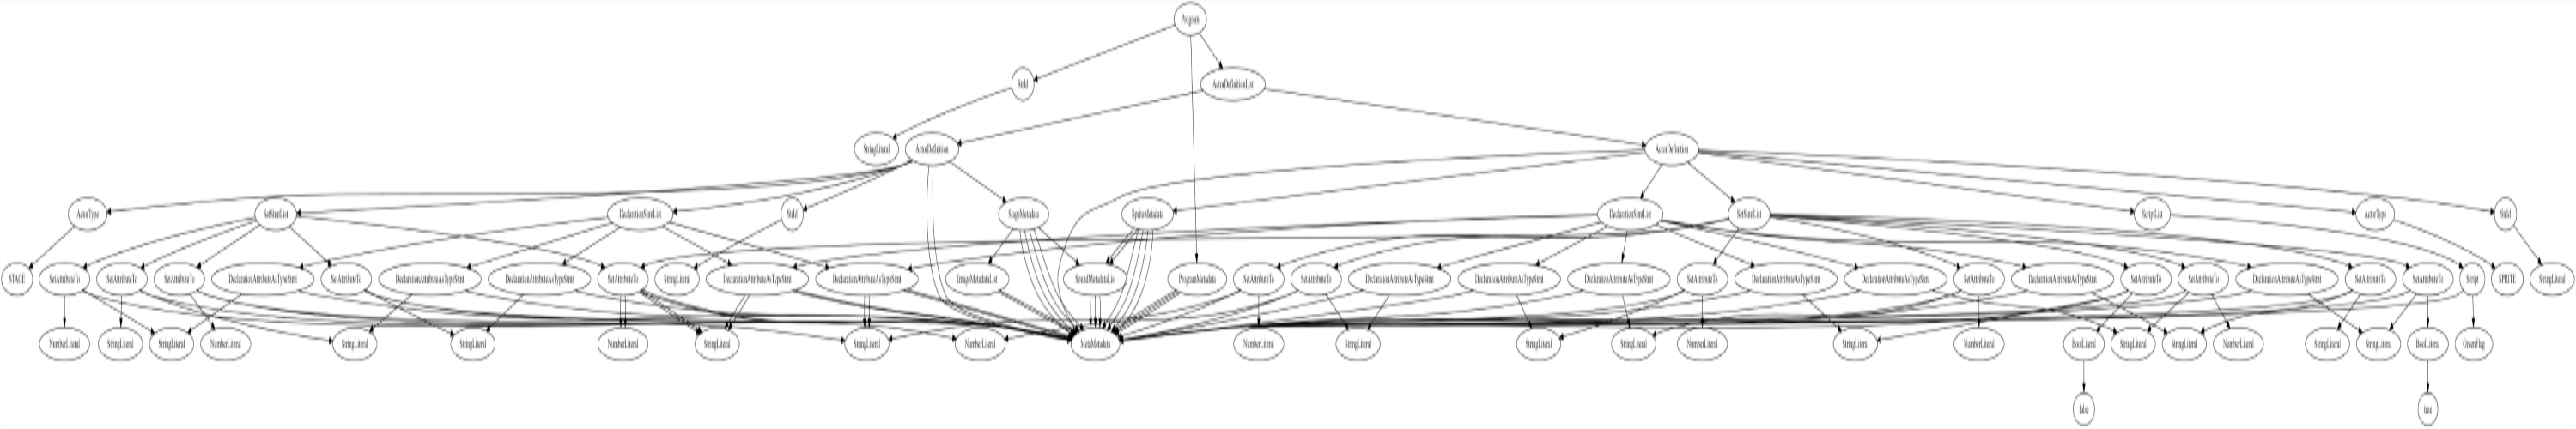
\includegraphics[scale=0.20]{images/AST_example(3).png}
\caption{Example AST structure of a simple \scratch\ project.}
\label{fig:ast}
\end{figure}

In order to identify unusual block sequences in a \scratch{} project, each project should be represented in the same form and structure. To visualise a \scratch{} project like it is shown in Figure~\ref{fig:ast}, the tokenization process is based on the abstract syntax tree (\AST{}) structure of \litterbox{}. 

For a simple \scratch{} project with only one [GreenFlag] block, the tree structure is already pretty big. This is caused by the number of additional information nodes that are created by the \litterbox{} \AST{} but are not necessary or even part of the essential tokens that are needed for an \ngram{}. In Table~\ref{tab:excluded-metadata} is a quick overview of all \AST{-only} nodes that are for information purposes, whereas in Table~\ref{tab:excluded-blocks} are real \scratch\ blocks that exist in the \AST\ that were excluded because of their usage in \textit{drop-down lists} only. It is assumed that a programmer cannot choose falsely in a \textit{drop-down list} and because the list itself can not be altered, all \textit{drop-down boxes} are seen as one  \hyperref[def:token]{\textit{token}} with their corresponding \scratch\ blocks. These nodes are all excluded for the tokenization in order to keep the n-gram model as small as possible and increase bug detection efficiency.  

\begin{figure}[hbtp]%
    \centering
    \subfloat[The script to tokenize.]{{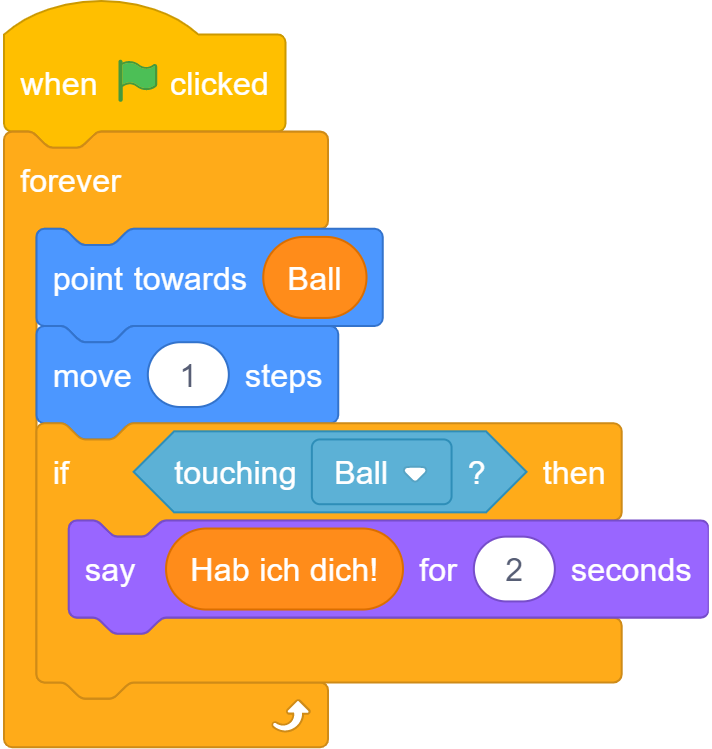
\includegraphics[width=7cm]{tokenization.png}\label{fig:tokenScript} }}%
    \qquad
    \subfloat[The tokens of the script.]{{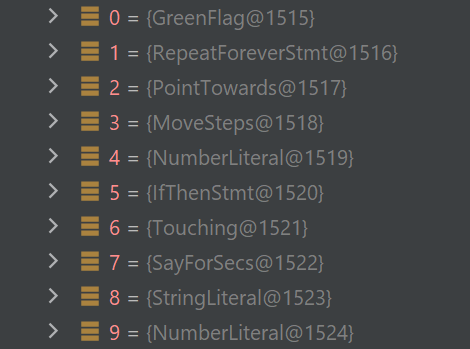
\includegraphics[width=7cm]{tokens.png}\label{fig:tokens} }}%
    \caption[Tokenization of a \scratch\ script]{\label{fig:tokenization}Tokenization of a \scratch\ script.}%
\end{figure}

As an example to show how a tokenized \scratch\ script looks like in the \tokenizer\ program, Figure~\ref{fig:tokenization} demonstrates how the partitioning into tokens works. While Subfigure~\ref{fig:tokenScript} visualises a solution script that was created for the \textit{Cat} task, the screenshot in Subfigure~\ref{fig:tokens} is a picture of the calculated tokens which do not always equal the original \scratch\ blocks because of their foundation in the \litterbox\ \AST{}. 

\begin{table}[hbtp]
    \caption[The from tokenization excluded information-based \AST\ nodes]{\label{tab:excluded-metadata}The excluded information-based \AST\ nodes for tokenization of \scratch\ projects.}

    \begin{tabular}[t]{lll}
    	\toprule
    	Class & Type & Example \\
    	\midrule
    	\vspace{10pt}
    	    \texttt{ActorDefinition} & \texttt{AbstractNode} & Information storage of actor \\
    	    \vspace{10pt} 
    	    \texttt{ActorDefinitionList} & \texttt{AbstractNode} & List of \texttt{ActorDefinition} \\
    	    \vspace{10pt}
        \texttt{ActorType} & \texttt{ASTLeaf} & \texttt{STAGE, SPRITE} \\  
        \vspace{10pt}
        \texttt{DeclarationStmt} & \texttt{Stmt} & All types of attribute declarations\\
        \vspace{10pt}
        \texttt{Metadata} & \texttt{ASTNode} & \parbox[t]{7cm}{Additional information of the\\ \texttt{Program, Sprites, Stages, Resources, Blocks}} \\
        \vspace{10pt}
        \texttt{ProcedureDefinition} & \texttt{AbstractNode} & Definition of custom procedures \\
        \vspace{10pt}
        \texttt{ProcedureDefinitionList} & \texttt{AbstractNode} & List of \texttt{ProcedureDefinition} \\
        \vspace{10pt}
        \texttt{Program} & \texttt{AbstractNode} & Placeholder for a project\\
        \vspace{10pt}
        \texttt{Script} & \texttt{AbstractNode} & \texttt{Event} and \texttt{StmtList} of an actor \\  
        \vspace{10pt}
        \texttt{ScriptList} & \texttt{AbstractNode} & List of \texttt{Script} \\
        \vspace{10pt}
        \texttt{SetAttributeTo} & \texttt{AbstractNode} & Sets attributes at start of program \\
        \vspace{10pt} 
        \texttt{SetStmtList} & \texttt{AbstractNode} & List of attributes to set \\
        \vspace{10pt}
        \texttt{StmtList} & \texttt{AbstractNode} & List of \texttt{Stmt} \\
        \vspace{10pt}
        \texttt{StrId} & \texttt{LocalIdentifier} & Project ID \\            
    \bottomrule
    \end{tabular}
\end{table}

\begin{table}[hbtp]
    \caption[The from tokenization excluded \scratch\ blocks]{\label{tab:excluded-blocks}The excluded \scratch\ blocks for tokenization.}

    \begin{tabular}[t]{lll}
    	\toprule
    	Class & Type & Examples \\
    	\midrule
    	\vspace{10pt}
    		\texttt{Position} & \texttt{ASTNode} & \texttt{MousePos, RandomPos} \\
    		\vspace{10pt} 
    		\texttt{Backdrop} & \texttt{AbstractNode} & Backdrop1, Backdrop2,... \\
    		\vspace{10pt} 
    		\texttt{Costume} & \texttt{AbstractNode} & Costume1, Costume2,... \\
    		\vspace{10pt}
    		\texttt{DragMode} & \texttt{ASTLeaf} & \texttt{Not\_DRAGGABLE, DRAGGABLE} \\
    		\vspace{10pt}
   		\texttt{ElementChoice} & \texttt{ASTNode} & \texttt{Next, Prev, Random, WithExpr} \\
   		\vspace{10pt}
    		\texttt{ForwardBackwardChoice} & \texttt{ASTLeaf} & \texttt{FORWARD, BACKWARD} \\
    		\vspace{10pt}
    		\texttt{GraphicEffect} & \texttt{ASTLeaf} & \texttt{COLOR, GHOST, BRIGHTNESS,...} \\
    		\vspace{10pt}
    		\texttt{Key} & \texttt{AbstractNode} & \texttt{Spacebar, Arrow keys, Any,...} \\
    		\vspace{10pt} 
   	 	\texttt{LayerChoice} & \texttt{ASTLeaf} & \texttt{FRONT, BACK} \\ 
   	 	\vspace{10pt}
    		\texttt{Loudness} & \texttt{NumExpr, ASTLeaf} & \texttt{Integer} \\
    		\vspace{10pt}
   		\texttt{Message} & \texttt{AbstractNode} & Message1, Message2,... \\
   		\vspace{10pt}
    		\texttt{NumFunct} & \texttt{ASTNode, ASTLeaf} & \texttt{ABS, ACOS, ASIN, ATAN,...} \\
    		\vspace{10pt} 
   		\texttt{Rotation-Style} & \texttt{ASTLeaf} & \parbox[t]{7cm}{\texttt{Don't rotate, Left-right,\\ All around}} \\
   		\vspace{10pt}
    		\texttt{Size} & \texttt{NumExpr, ASTLeaf} & \texttt{Integer} \\
    		\vspace{10pt}
    		\texttt{SoundEffect} & \texttt{ASTLeaf} & \texttt{PAN, PITCH} \\
    		\vspace{10pt}
    		\texttt{TimeComp} & \texttt{ASTNode, ASTLeaf} & \texttt{DATE, DAY\_OF\_WEEK, HOUR,...} \\
    		\vspace{10pt}
    		\texttt{Timer} & \texttt{NumExpr, ASTLeaf} & \texttt{Integer} \\
    		\vspace{10pt} 
    		\texttt{Touchable} & \texttt{ASTNode} & \parbox[t]{7cm}{\texttt{Color, MousePointer, SpriteTouchable, Edge}} \\
    		\vspace{10pt}
    		\texttt{Variable} & \texttt{DataExpr} & My variable \\ 
    		\vspace{10pt}
        \texttt{Volume} & \texttt{NumExpr, ASTLeaf} & \texttt{Integer} \\     
    \bottomrule
    \end{tabular}
\end{table}


\section{N-gram Model Building in \scratch{}}\label{sec:model}
In the following sections the focus is on the building process of the \ngram{}, specifically in \scratch{}. Subsection~\ref{subsec:n-grams} goes in detail on how to calculate the probabilities of the found \hyperref[def:token]{\textit{token}} sequences and add them to the growing model. The method of \hyperref[def:smoothing]{\textit{Smoothing}} is then explained in Subsection~\ref{subsec:smoothing} as well as its importance in bug detection.

\subsection{Calculating and Adding N-grams}\label{subsec:n-grams}
First of all, the language model has to extract all possible \hyperref[def:token]{\textit{token}} sequences in a \scratch{} project and calculate their probabilities like it is described in Subsection~\ref{subsec:n-grams}. This way a reliable probability distribution is created that will be the basis for later bug detection. 

For example, given the sequence [GreenFlag, Show, Hide] that is shown in Figure~\ref{fig:sequence}, all its consecutive subsequences are added to the model. In this case the subsequence [GreenFlag, Hide] that is shown in Figure~\ref{fig:subsequence} would be the only sequence that is ignored because [Hide] does not immediately follow [GreenFlag]. 

\begin{figure}[hbtp]%
    \centering
    \subfloat[A \scratch{} block sequence.]{{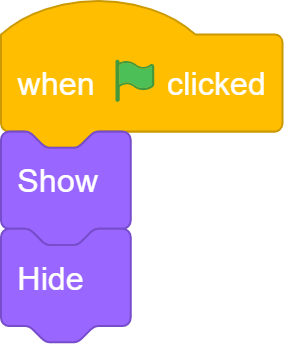
\includegraphics[width=5cm]{sequence.png} }\label{fig:sequence}}%
    \qquad
    \subfloat[Ignored subsequence.]{{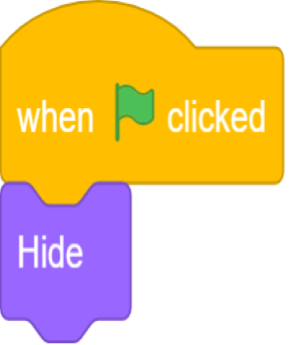
\includegraphics[width=5cm]{subsequence.png} }\label{fig:subsequence}}%
    \caption[\scratch{} block sequences]{\label{fig:sequences}\scratch{} block sequences.}%
\end{figure}

If Figure~\ref{fig:sequence} would be the sequence we want to calculate the probability of, the estimation based on the \hyperref[def:markov_chain]{\textit{Markov chain}} is executed by solving the Equation~\ref{eq:scratch-prob}. We are setting the \hyperref[def:gram size]{\textit{gram size}} to 3 in this example. All internal probabilities are added by consulting the existing model and searching for the already calculated estimations. Therefore, the token sequence [GreenFlag, Show, Hide] can be calculated based on internal probabilities of its existing subsequences.

\begin{equation} \label{eq:scratch-prob}
\begin{aligned}
P([GreenFlag, Show, Hide]) ={} & P([GreenFlag])\cdot P([Show]|[GreenFlag]) \\
							  & \cdot P([Hide]|[GreenFlag, Show])
\end{aligned}
\end{equation}


\subsection{Smoothing of Probability Distribution}\label{subsec:smoothing}

\begin{definition}[Smoothing]\label{def:smoothing}
	%
	``In mathematics 'smoothing' means to free a graph, a collection of data, etc. from irregularities.''~\cite{smoothing}
	%
\end{definition}

If the analysed project is not part of the training data set, it is important to smooth the probability distribution in order to avoid probabilities of zero. In this implementation, \textit{Add-One-Smoothing} was utilized which prevents non existent sequences to be shown by adding an additional count to each n-gram. All the counts that used to be zero will now have a count of 1, the counts of 1 will be 2, and so on. This algorithm is also called \textit{Laplace Smoothing}. This way there are no sequences with a probability of zero stored in the model that could affect the calculation of the sequence probabilities.

In the case of the unigram [GreenFlag], its maximum likelihood to appear in a \scratch{} project is estimated by counting the occurrences \textit{c} during the model training process and divide it through the total number of tokens \textit{N}. Therefore, the Equation~\ref{eq:likelihood} looks like this:

\begin{equation} \label{eq:likelihood}
P([GreenFlag]) ={} \frac{c}{N}
\end{equation}

\textit{Add-One-Smoothing} then, like the name suggests, only adds one to each count. Since there are a total of \textit{D} tokens in the model vocabulary and we added one more sighting to each one of them, we also have to adjust the denominator of the fraction accordingly. One more observation of each \hyperref[def:token]{\textit{token}} means we have to increase the denominator by \textit{D}. If we apply the mathmatic rules accordingly, the equation results in the following calculation in Equation~\ref{eq:laplace}:

\begin{equation} \label{eq:laplace}
P_{Laplace}([GreenFlag]) ={} \frac{c + 1}{N + D}
\end{equation}


\section{Bug Detection in \scratch{}}\label{sec:detection}
The specific algorithm to find bugs in \scratch{} is implemented the following way. At first, the probabilities of all sequences of the analysed project have to be calculated with help of the model, like it is described in Subsection~\ref{subsec:n-grams}. After that, the sequences are ranked based on their probability and only the ones with the lowest probability get reported as potential bugs. In the next Subsection~\ref{subsec:configurations} all important parameters are set to ensure the optimal model analysis results. In Subsection~\ref{subsec:false_bugs} we found a method to minimize the number of false positives in the reported bug set.

\subsection{Configurations}\label{subsec:configurations}
For the \scratch{} model implementation we added five parameters that have to be set accordingly in order to achieve the best evaluation results that are discussed later in Chapter~\ref{chap:evaluation}.

\paragraph{\hyperref[def:gram_size]{Gram Size.}}
For probability calculations a \hyperref[def:markov_chain]{\textit{Markov chain}} is used to get the conditional probability of a sequence using its n - 1 \hyperref[def:token]{\textit{token}} predecessors as context information. In this work, the \hyperref[def:gram_size]{\textit{gram size}} is adopted from the \bugram{}~\cite{bugram} paper where the value of 3 had the best results. 

\paragraph{\hyperref[def:sequence_length]{\textit{Sequence Length.}}}
In order to analyse \scratch\ projects on a rather small granularity level, we utilized \hyperref[def:sequence_length]{\textit{sequence lengths}} of 2 and 3 in our implementation after analysing the results of multiple combinations of \hyperref[def:sequence_length]{\textit{sequence lengths}}. Together with the \hyperref[def:gram_size]{\textit{gram size}} of 3, these \hyperref[def:sequence_length]{\textit{sequence lengths}} are effective in partitioning the \scratch\ programs into pieces that give back useful probabilities. The usage of two different \hyperref[def:sequence_length]{\textit{sequence lengths}} also ensures that the reported bugs are at the bottom of at least two analysing n-gram models. This method reduces the number of false positives that would otherwise occur more frequently.

\paragraph{\hyperref[def:reporting_size]{Reporting Size.}}
We did not limit the \hyperref[def:reporting_size]{\textit{reporting size}} for the small data set that is further introduced in Subsection~\ref{subsec:bugset}. The number of reported bugs is very small in the case of the data set because the projects as well as the model itself are not very big. If we would have restricted the number of reported bugs even more, there would not be enough output created to analyse.  

\paragraph{\hyperref[def:minimum_token_occurrence]{Minimum Token Occurrence.}}
In this bachelor's thesis the \hyperref[def:minimum_token_occurrence]{\textit{minimum token occurrence}} is chosen as 1. Because of the size difference between usual \java\ projects compared to normal \scratch{} projects, it would not be helpful to filter out any tokens. \scratch{} programmers do not have as much freedom in their implementation because of the restrictions of a block-based language and usually choose a different purpose for their programs than text-based programming languages would, which leads to much smaller projects with fewer usages of specific tokens. So, the \hyperref[def:minimum_token_occurrence]{\textit{minimum token occurrence}} parameter would only make it harder to find low probability sequences in projects which is why we decided not to raise this threshold for the analysis.

\paragraph{\hyperref[def:probability_threshold]{Probability Threshold.}}
The \hyperref[def:probability_threshold]{\textit{probability threshold}} is determined individually for each \ngram\ by examining the reported sequences of a few example projects, categorizing the true bugs and choosing a probability value that is low enough to detect the most true bugs with a minimum number of false positives. Every sequence with a higher probability is then considered a normal sequence that can not be reported as a bug because its occurrence rate is too high. In this implementation, the threshold is fixed at 0.05\% for the big data set of Subsection~\ref{subsec:trainingset} and at 0.5\%, 0.6\% or 1.6\% for the pupils' projects of Subsection~\ref{subsec:bugset}. 

\subsection{Pruning False Bugs}\label{subsec:false_bugs}
\hyperref[def:token]{\textit{Token}} sequences with low probabilities are at the bottom of an n-gram reporting list for potential bugs. But there is always the chance that the found sequence is not actually wrong but just a very unusual or special use case in which its probability would also rank rather low. To find and filter out this kind of false bugs and reduce the candidate bug set, \hyperref[def:token]{\textit{token}} sequences can only be reported when they are at the bottom of at least two ranked lists of \ngram{s} with the same \hyperref[def:gram_size]{\textit{gram size}} but different \hyperref[def:sequence_length]{\textit{sequence lengths}}. This way, sequences are sorted out that just appear on one of these lists and the chance to report false positives gets drastically reduced. 


\section{Implementation}\label{sec:implementation}
This section explains the tool chain of our approach for \ngram{} in \scratch\ and clarifies implementation
decisions. Table~\ref{tab:ngram-params} gives an overview over the model building process in \scratch, the bug detection system, the parameters which can be adjusted, and the input and output of each step.

\begin{table}[H]
    \caption[The tool chain for n-gram bug detection in \scratch]{\label{tab:ngram-params}The tool chain for n-gram bug detection in \scratch.}

    \begin{tabular}[t]{lllll}
        \toprule
        \parbox{2cm}{Steps} & Input & Tool & \parbox{2cm}{Output\\format} & Parameters \\
        \midrule
        \vspace{10pt}
        
        \parbox[t]{2cm}{Model\\ Building} &\parbox[t]{2.5cm}{\scratch\ data set,\\ \texttt{model.csv}} & \parbox[t]{3cm}{\ngramtrainer{}, \tokenizer{}} & \parbox[t]{2cm}{\texttt{.csv}} & \parbox[t]{3.8cm}{\hyperref[def:gram_size]{gram size}}\\
        
        \vspace{10pt}
        
        \parbox[t]{2cm}{Bug\\ Detection} & \parbox[t]{2.5cm}{\scratch\ \\ bug set,\\ \texttt{model.csv},\\ \texttt{report.csv}} & \parbox[t]{3cm}{\ngrambugfinder{}, \tokenizer{}} & \parbox[t]{2cm}{\texttt{.csv}} & \parbox[t]{3.8cm}{\hyperref[def:reporting_size]{report size},\\ \hyperref[def:gram_size]{gram size},\\ 	\hyperref[def:sequence_length]{sequence length},\\ \hyperref[def:probability_threshold]{probability \\ threshold},\\ with/without \hyperref[def:smoothing]{smoothing}}\\ 

        \bottomrule
    \end{tabular}
\end{table}

\subsection{\tokenizer{}}\label{subsec:tokenizer}
The basis of the n-gram building process is to tokenize each project and structure it in the same way. The \ngramtrainer\ as well as \ngrambugfinder\ both use \litterbox\ to create an \AST\ for a given program. The \AST\ then maps every command block to a corresponding \AST\ node. In this process every \textit{hat block} is implementing the interface \texttt{Event} and all remaining \textit{command blocks} are associated with the \texttt{Stmt} interface. For instance, the [Turn Right] block is represented by an object of the \texttt{TurnRight} class which implements the \texttt{Stmt} interface. A visitor then visits the \AST\ and partitions the project into its \hyperref[def:token]{tokens}.

\subsection{\ngramtrainer{}}\label{subsec:ngramtrainer}
\ngramtrainer{}, a feature added to \litterbox{}, creates an \ngram\ based on a set of \scratch\ projects. The model stores a probability distribution for all \hyperref[def:token]{\textit{token}} sequences that were found in the training set. It is then utilized as a foundation for bug detection in \scratch{}.

The model creation process consists of three steps: At first, all possible sequences of tokens that can be created from the analysed training set are calculated, counted, and stored in a \texttt{Map} structure. Then we go through the \texttt{Map} of sequences and estimate the probability of each sequence, like it is shown in Equation~\ref{eq:likelihood}, by counting the amount a sequence appeared during the n-gram calculation and dividing it by the total number of sequences. After the calculation a finished model is printed as a \texttt{.csv} file and is ready for its usage in further analysis and bug detection procedures.

\subsection{\ngrambugfinder{}}\label{subsec:ngrambugfinder}
\ngrambugfinder{}, another extension that was added to \litterbox{}, continues the analysis process of the \ngramtrainer\ by using its calculated model. First, to find bugs in a project, the project itself is partitioned into sequences of a specific length that are stored in a \texttt{Map}. Then the probability of each sequence is estimated with help of the given probability distribution of the n-gram model. The probabilities are then ranked and the sequences with the lowest scores are reported as potential bugs. The final \texttt{.csv} file then shows the reported sequences with their location information and calculated probabilities.